\chapter{Additional Design Diagrams}
The main use-case, architecture, domain/schema, sequence and deployment diagrams are in Chapters 4--6. This appendix contains supporting data-flow, activity, state, layering and future-wireframe models. All are editable TikZ sources.
\begin{figure}[htbp]\centering\begin{minipage}{.82\linewidth}\resizebox{\linewidth}{!}{\begin{tikzpicture}[x=1mm,y=1mm,b/.style={draw,rounded corners,text width=49mm,minimum height=24mm,align=center,font=\sffamily\footnotesize},store/.style={draw,double,text width=49mm,minimum height=19mm,align=center,font=\sffamily\footnotesize},>=Stealth]
\node[b] (user) at (75,146){User: selection, answers and candidate};\node[b] (loader) at (32,106){P1: load/validate\\Case + source identity};\node[b] (profile) at (118,106){P2: score profile/policy\\Capacity, tolerance, allowance};
\node[b] (check) at (32,61){P3: verify claims\\Candidate and source independently};\node[b] (emit) at (118,61){P4: emit current result\\Accepted, fallback or error};
\node[store] (files) at (32,13){D1: recorded artifacts / receipts};\node[store] (state) at (118,13){D2: session profile / result identity};
\draw[->](user.south)-|node[pos=.35,above,font=\scriptsize]{case/text}(loader.north);\draw[->](user.south)-|node[pos=.35,above,font=\scriptsize]{18 answers}(profile.north);
\draw[->](files.west)--(-5,13)--node[left,font=\scriptsize]{record}(-5,106)--(loader.west);\draw[->](loader)--(check);\draw[->](check)--node[above,font=\scriptsize]{verdict}(emit);\draw[->](profile)--node[right,font=\scriptsize]{policy result}(emit);\draw[->](emit)--(state);
\draw[->](emit.east)--(153,61)--(153,146)--node[above,font=\scriptsize]{current display}(user.east);
\end{tikzpicture}}
\end{minipage}\caption{Data flow through case, profile and explanation checks.}\label{fig:dataflow}\end{figure}
\begin{figure}[htbp]\centering\resizebox{\linewidth}{!}{\begin{tikzpicture}[x=1mm,y=1mm,b/.style={draw,rounded corners,text width=48mm,minimum height=15mm,align=center,font=\sffamily\footnotesize},d/.style={draw,diamond,aspect=2.5,align=center,font=\sffamily\scriptsize,inner sep=1mm},>=Stealth]
\node[circle,fill,minimum size=3mm,inner sep=0] (start) at (75,192){};
\node[b] (load) at (75,175){Load and validate selected record};\node[d] (valid) at (75,151){Valid?};
\node[b] (candidate) at (75,126){Read current text/payload; verify independently};\node[d] (pass) at (75,101){Candidate passes?};
\node[b] (accept) at (28,76){Emit candidate and accepted report};\node[b] (fallback) at (122,76){Retain rejection; render fallback};
\node[d] (fallbackpass) at (122,46){Fallback passes?};\node[b] (emit) at (76,18){Emit checked replacement};\node[b] (error) at (20,18){Show error; no verified output};
\node[circle,draw,double,fill=black,minimum size=4mm,inner sep=0] (end) at (75,-11){};
\draw[->](start)--(load);\draw[->](load)--(valid);\draw[->](valid)--node[right]{yes}(candidate);\draw[->](candidate)--(pass);
\draw[->](valid.west)--node[above]{no}(-15,151)--(-15,18)--(error.west);
\draw[->](pass.west)-|node[pos=.25,above]{yes}(accept.north);\draw[->](pass.east)-|node[pos=.25,above]{no}(fallback.north);
\draw[->](fallback)--(fallbackpass);\draw[->](fallbackpass.south)|-node[pos=.25,above]{yes}(emit.east);
\draw[->](fallbackpass.east)--node[above]{no}(154,46)--(154,0)--(20,0)--(error.south);
\draw[->](accept.south)--(28,55)--(-30,55)--(-30,-11)--(end.west);
\draw[->](emit.south)--(end.north);\draw[->](error.south)|-(end.west);
\end{tikzpicture}}
\caption{Checking activity and failure branches.}\label{fig:activity}\end{figure}
\begin{figure}[htbp]\centering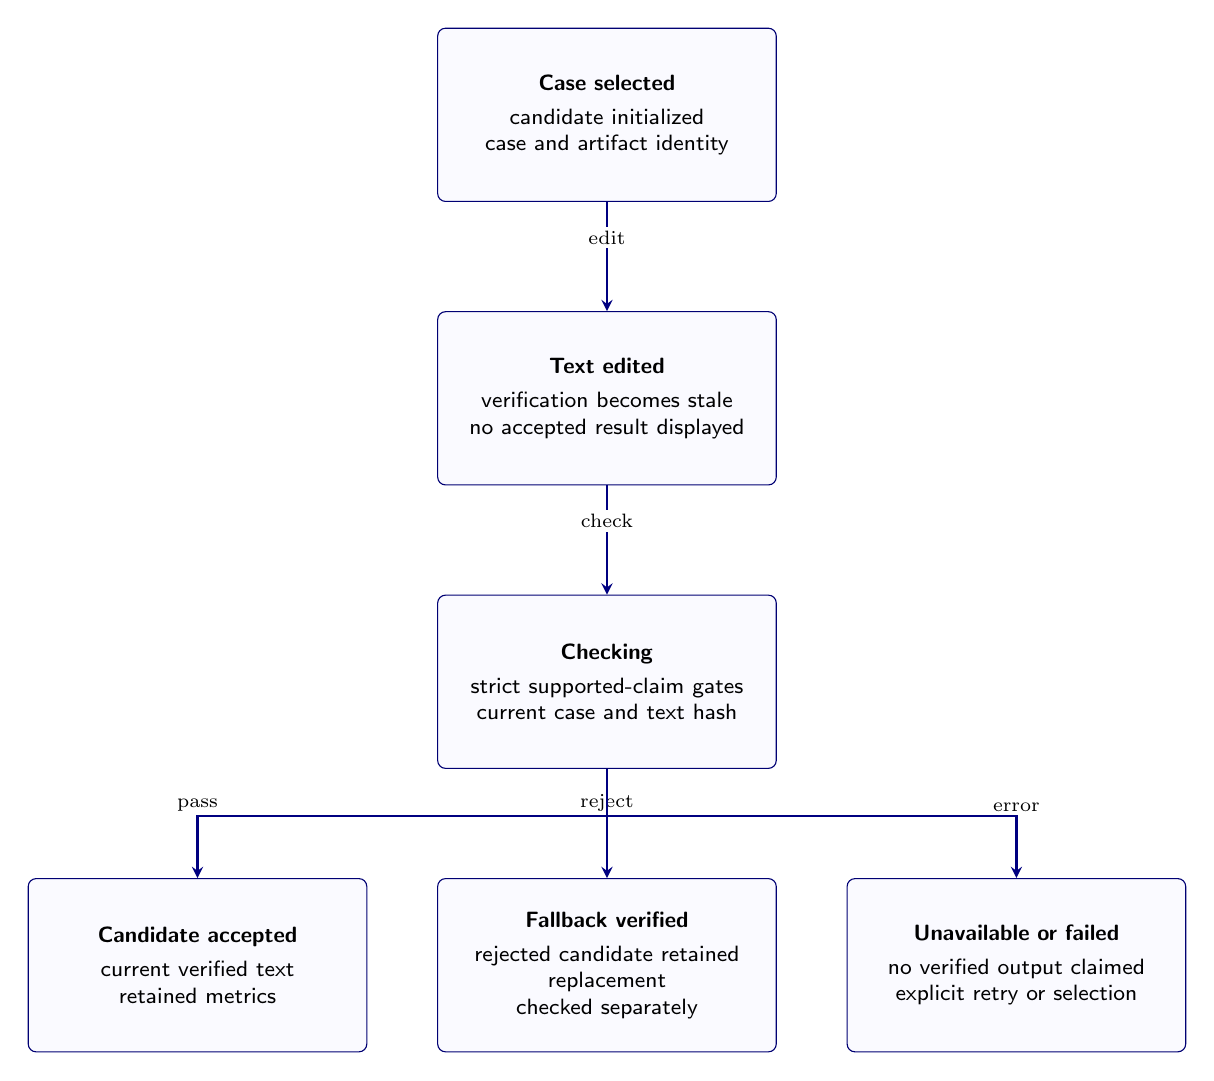
\begin{tikzpicture}[x=1mm,y=1mm,box/.style={draw=blue!45!black,fill=blue!2,rounded corners=1mm,align=center,text width=39mm,minimum height=22mm,inner sep=2mm,font=\sffamily\footnotesize},link/.style={->,>=stealth,draw=blue!50!black,thick}]
\node[box] (selected) at (75,135) {\textbf{Case selected}\\[1mm]candidate initialized\\case and artifact identity};
\node[box] (edited) at (75,99) {\textbf{Text edited}\\[1mm]verification becomes stale\\no accepted result displayed};
\node[box] (checking) at (75,63) {\textbf{Checking}\\[1mm]strict supported-claim gates\\current case and text hash};
\node[box] (accepted) at (23,27) {\textbf{Candidate accepted}\\[1mm]current verified text\\retained metrics};
\node[box] (fallback) at (75,27) {\textbf{Fallback verified}\\[1mm]rejected candidate retained\\replacement checked separately};
\node[box] (error) at (127,27) {\textbf{Unavailable or failed}\\[1mm]no verified output claimed\\explicit retry or selection};
\draw[link] (selected.south) -- ++(0,-6) -| (edited.north) node[pos=.5,above,fill=white,inner sep=.5mm,font=\scriptsize]{edit};
\draw[link] (edited.south) -- ++(0,-6) -| (checking.north) node[pos=.5,above,fill=white,inner sep=.5mm,font=\scriptsize]{check};
\draw[link] (checking.south) -- ++(0,-6) -| (accepted.north) node[pos=.5,above,fill=white,inner sep=.5mm,font=\scriptsize]{pass};
\draw[link] (checking.south) -- ++(0,-6) -| (fallback.north) node[pos=.5,above,fill=white,inner sep=.5mm,font=\scriptsize]{reject};
\draw[link] (checking.south) -- ++(0,-6) -| (error.north) node[pos=.5,above,fill=white,inner sep=.5mm,font=\scriptsize]{error};
\end{tikzpicture}
\caption{Verification state and stale-result invalidation.}\label{fig:state}\end{figure}
\begin{figure}[htbp]\centering\resizebox{\linewidth}{!}{\begin{tikzpicture}[x=1mm,y=1mm,b/.style={draw,text width=135mm,minimum height=23mm,align=center,font=\sffamily\footnotesize},>=Stealth]
\node[b] (ui) at (75,119){\textbf{Presentation}\\Overview / Decision / Evidence / Risk / Explanation / Studies};
\node[b] (app) at (75,81){\textbf{Application}\\Case loading, current-state ownership, confidence policy and emission};
\node[b] (domain) at (75,43){\textbf{Domain}\\Validated records, feature meanings, tolerance/capacity and claim checks};
\node[b] (files) at (75,5){\textbf{Artifacts / runtime}\\Versioned JSON traces, original models, study receipts and local session memory};
\draw[->](ui)--node[right,font=\scriptsize]{user action}(app);\draw[->](app)--node[right,font=\scriptsize]{validated contract}(domain);\draw[->](domain)--node[right,font=\scriptsize]{read / retain identity}(files);
\end{tikzpicture}}
\caption{Current presentation, application, domain and storage layers.}\label{fig:layers}\end{figure}
\begin{figure}[htbp]\centering\resizebox{\linewidth}{!}{\begin{tikzpicture}[x=1mm,y=1mm,b/.style={draw,rounded corners,text width=60mm,minimum height=45mm,align=left,font=\sffamily\footnotesize,inner sep=2mm},>=Stealth]
\node[b] (onboard) at (34,156){\textbf{1. Onboarding}\\Educational purpose / limits\\Data and privacy controls\\Start analysis};
\node[b] (profile) at (116,156){\textbf{2. Profile}\\Capacity + 13 tolerance items\\Binding tier / risk allowance\\Required confidence};
\node[b] (company) at (116,88){\textbf{3. Company selection}\\Audited company universe\\Data-age/coverage status\\Choose horizon};
\node[b] (decision) at (34,88){\textbf{4. Decision and evidence}\\Qualified signal or abstention\\Probability / SHAP / inputs\\Open feature detail};
\node[b] (check) at (34,20){\textbf{5. Explanation/checking}\\User-facing explanation\\Claim report and recovery\\Explicit confidence limitations};
\node[b,dashed] (chat) at (116,20){\textbf{6. Follow-up (planned)}\\Question about current evidence\\Rolling context / citations\\Source-bound verified response};
\draw[->](onboard)--(profile);\draw[->](profile)--(company);\draw[->](company)--(decision);\draw[->](decision)--(check);\draw[->,dashed](check)--(chat);
\node[align=center,font=\scriptsize,text width=143mm] at (75,-23){Wireframes describe the product journey. Dashed follow-up and multi-company/service integrations are future scope; actual screenshots are shown separately.};
\end{tikzpicture}}
\caption{Planned full-product interfaces; not completed software.}\label{fig:final-wireframes}\end{figure}
